\begingroup
\let\figure\RSIappendixfigure
\let\endfigure\RSIendappendixfigure
\subsubsection{Original four-round Qwen3-4B figures}
\label{app:qwen4b-raw-figures}

Figures~\ref{fig:qwen4b-raw-unaudited}--\ref{fig:qwen4b-raw-comparison-difficulty}
present the Qwen3-4B trajectories in the same six groups as
Appendix~\ref{app:qwen-raw-figures}: unaudited, audited, and joint
comparisons, each with aggregate and difficulty-stratified views.
The separate-policy plots are original exports; the joint views are
generated from the same checkpoint records with the same plotting method.
They complement Figure~\ref{fig:graph-four-round}(c--d) and
Table~\ref{tab:qwen4b-endpoints}, not additional experiments.
All use five paired blocks and fixed sets of 2,000 ID or 1,000 OOD
questions. Error bars are pointwise, descriptive 95\% block-$t$ intervals.

\begin{figure}[H]
\centering
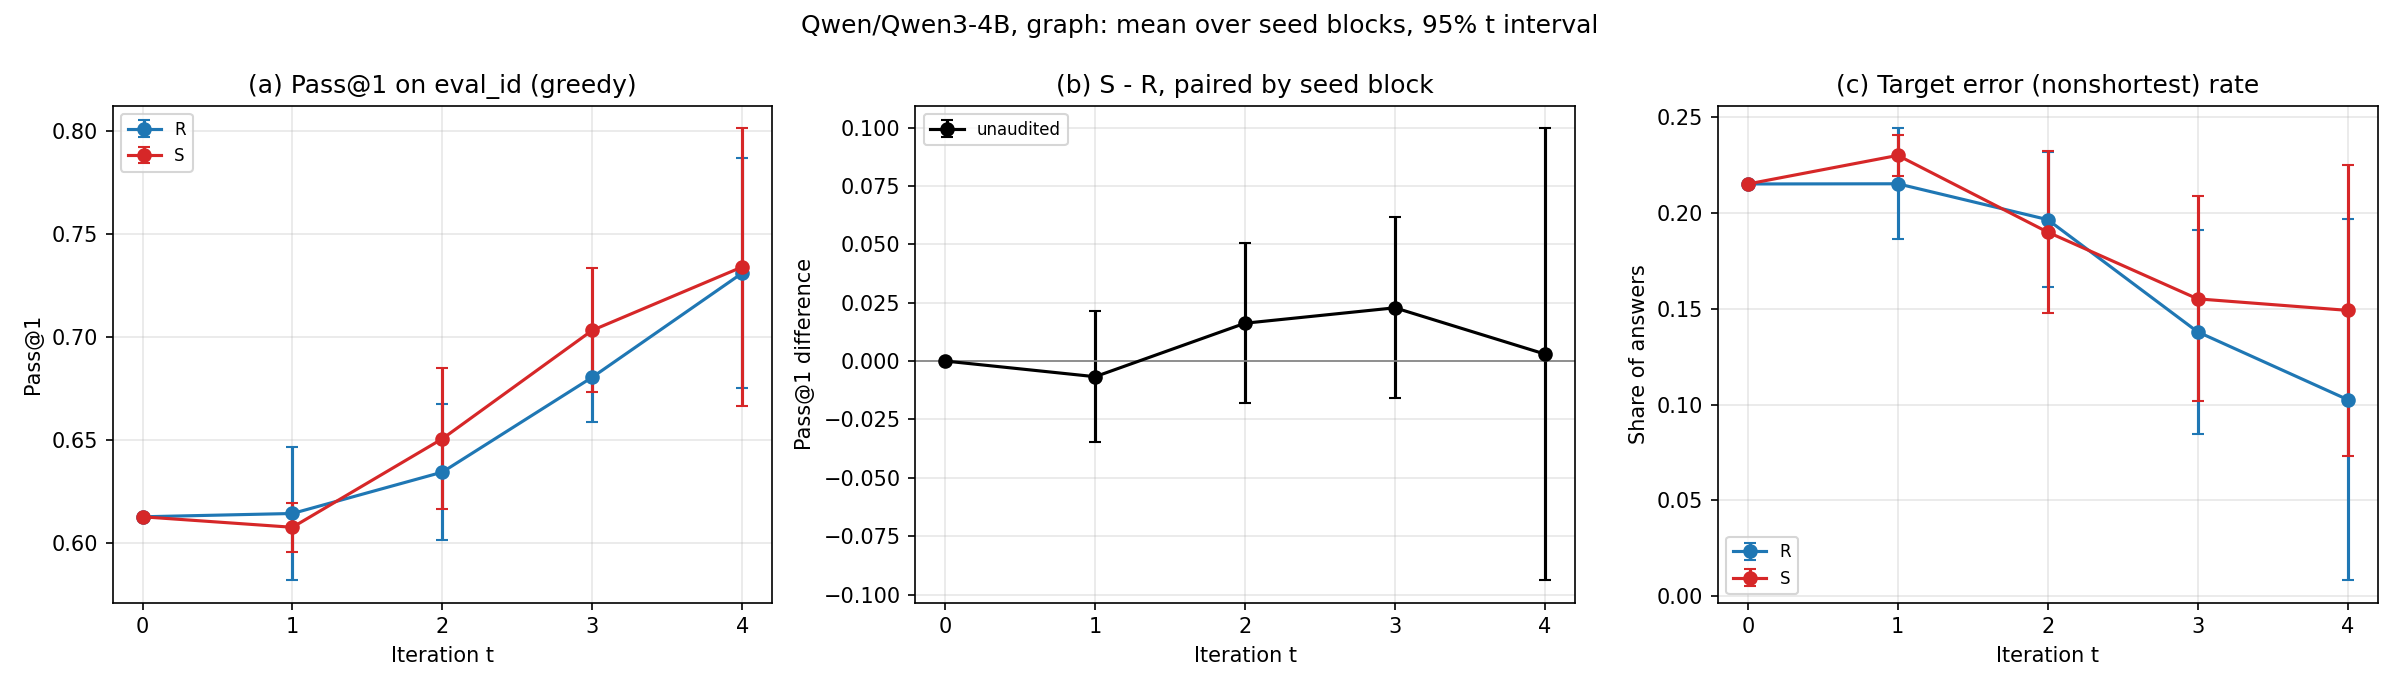
\includegraphics[width=0.90\linewidth]{figures/qwen4b_four_round_raw/unaudited_eval_id_pass1.png}
\par\smallskip
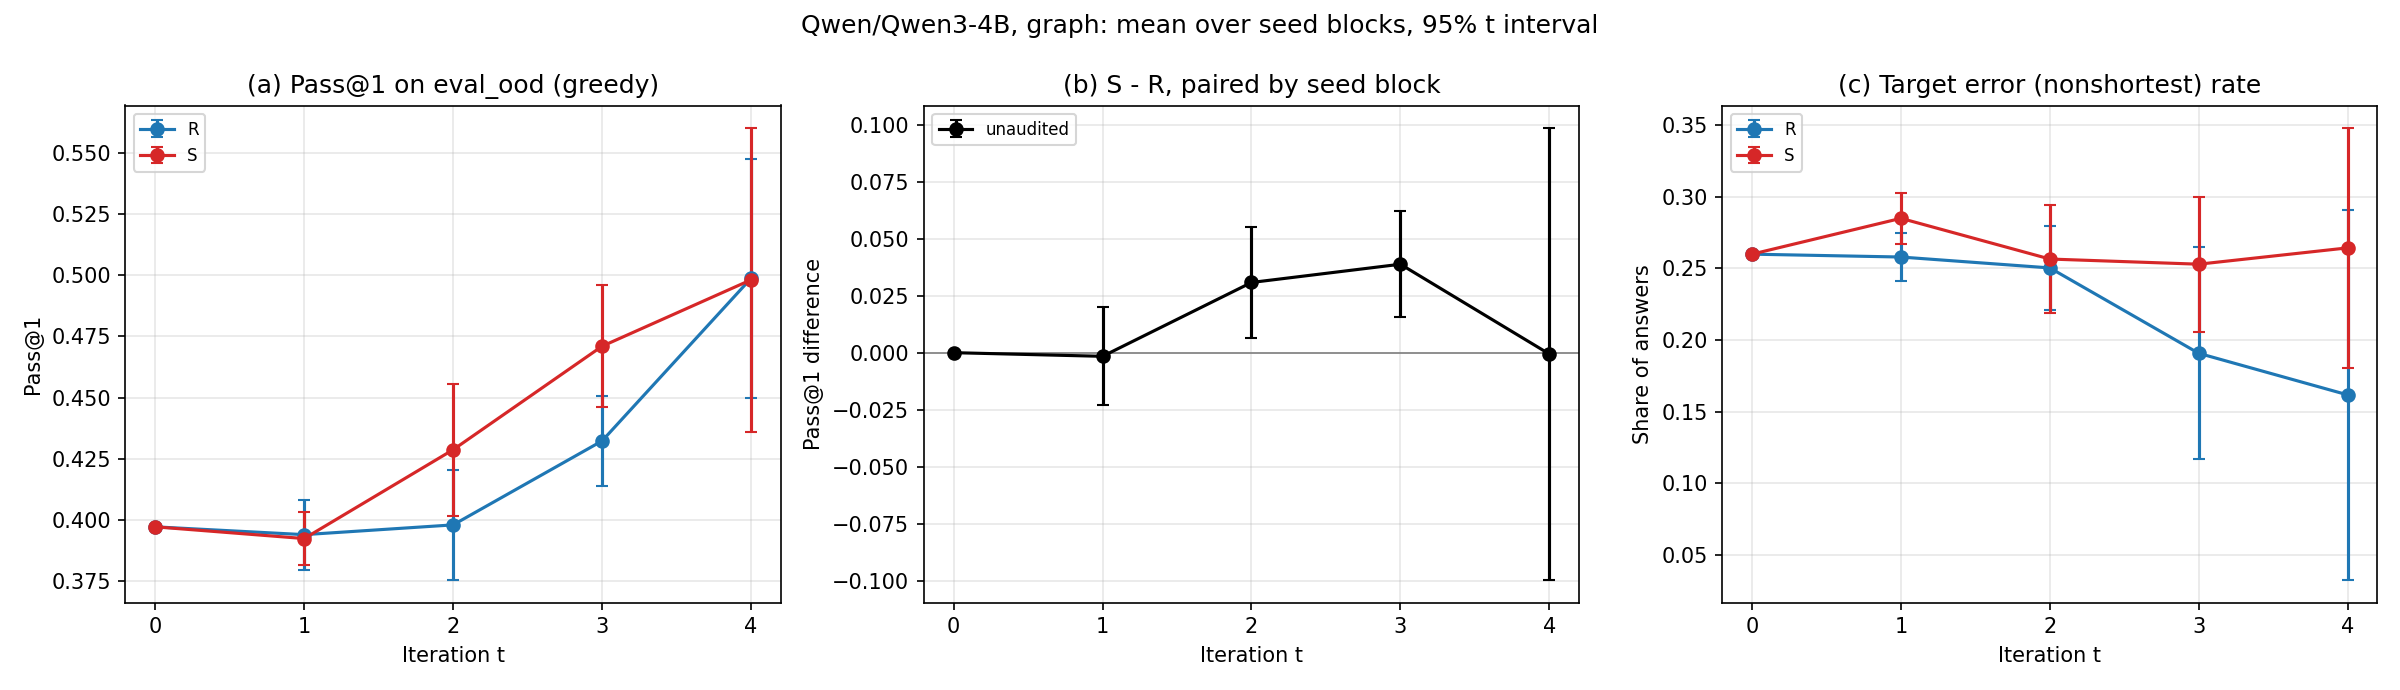
\includegraphics[width=0.90\linewidth]{figures/qwen4b_four_round_raw/unaudited_eval_ood_pass1.png}
\caption{Original unaudited Qwen3-4B graph curves, ID (top) and OOD
(bottom), for rounds 0--4. The panels show greedy Pass@1, paired
$S-R$ accuracy, and nonshortest-error incidence among all answers.}
\label{fig:qwen4b-raw-unaudited}
\end{figure}

Unaudited $R/S$ accuracy reaches $0.7309/0.7339$ ID and
$0.4988/0.4982$ OOD, from bases $0.6125$ and $0.3970$.
Paired endpoint contrasts are $0.0030\pm0.0968$ ID and
$-0.0006\pm0.0991$ OOD. The positive mean OOD contrast in
intermediate rounds declines to near zero at the endpoint.

\begin{figure}[H]
\centering
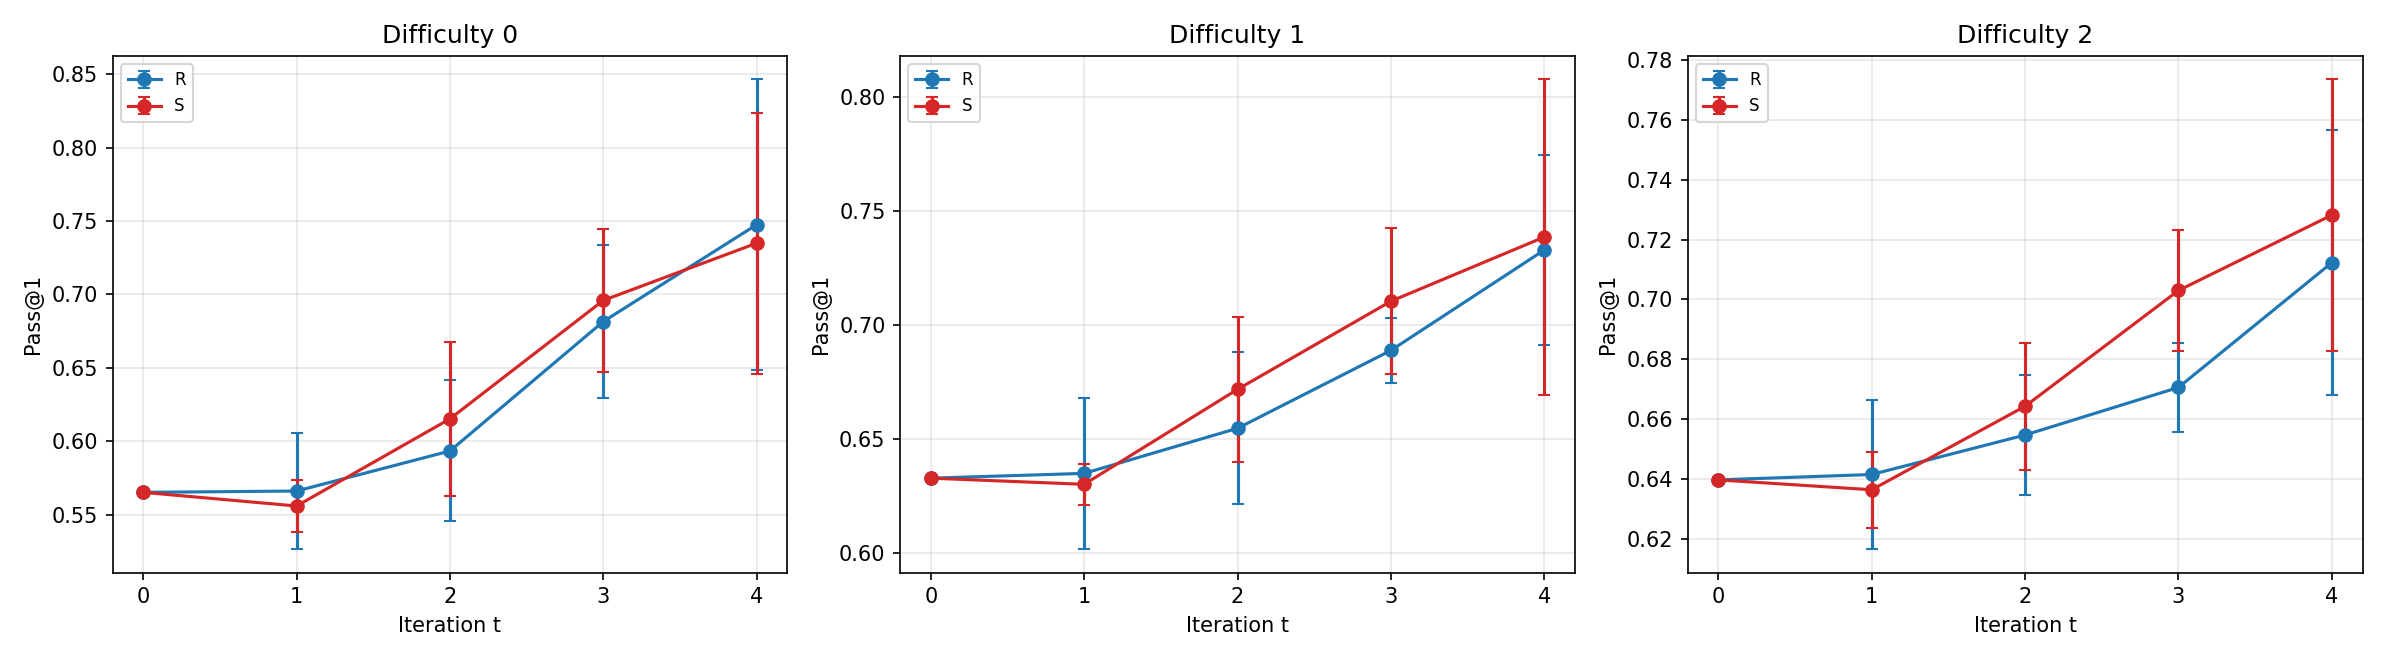
\includegraphics[width=0.90\linewidth]{figures/qwen4b_four_round_raw/unaudited_eval_id_by_difficulty.png}
\par\smallskip
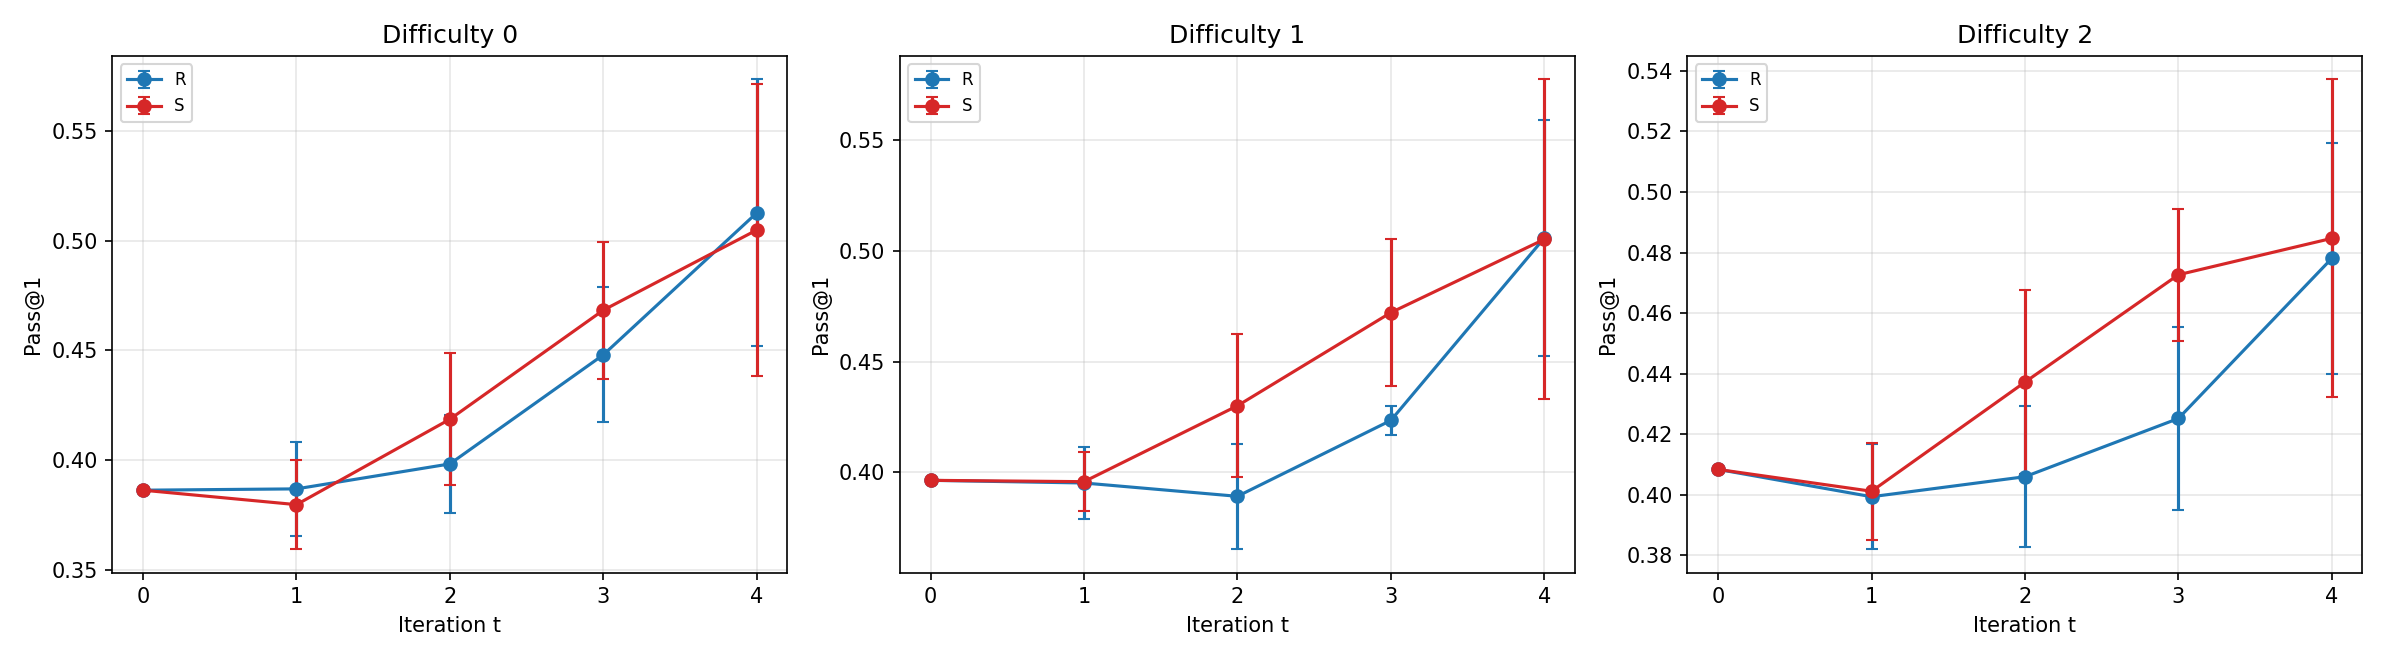
\includegraphics[width=0.90\linewidth]{figures/qwen4b_four_round_raw/unaudited_eval_ood_by_difficulty.png}
\caption{Original unaudited Qwen3-4B graph accuracy by generator
difficulty stratum, ID (top) and OOD (bottom), for rounds 0--4.
Strata 0--2 appear from left to right, containing $667/667/666$ ID
and $334/333/333$ OOD questions. Intervals use the same five blocks
as Figure~\ref{fig:qwen4b-raw-unaudited}.}
\label{fig:qwen4b-raw-unaudited-difficulty}
\end{figure}

The fixed generator strata do not establish a model-difficulty ordering.
Panel-specific vertical scales are retained, and these comparisons are
descriptive rather than multiplicity-adjusted. The breakdown provides
context for the aggregate trajectory without adding a stratum-level
accuracy claim.

\begin{figure}[H]
\centering
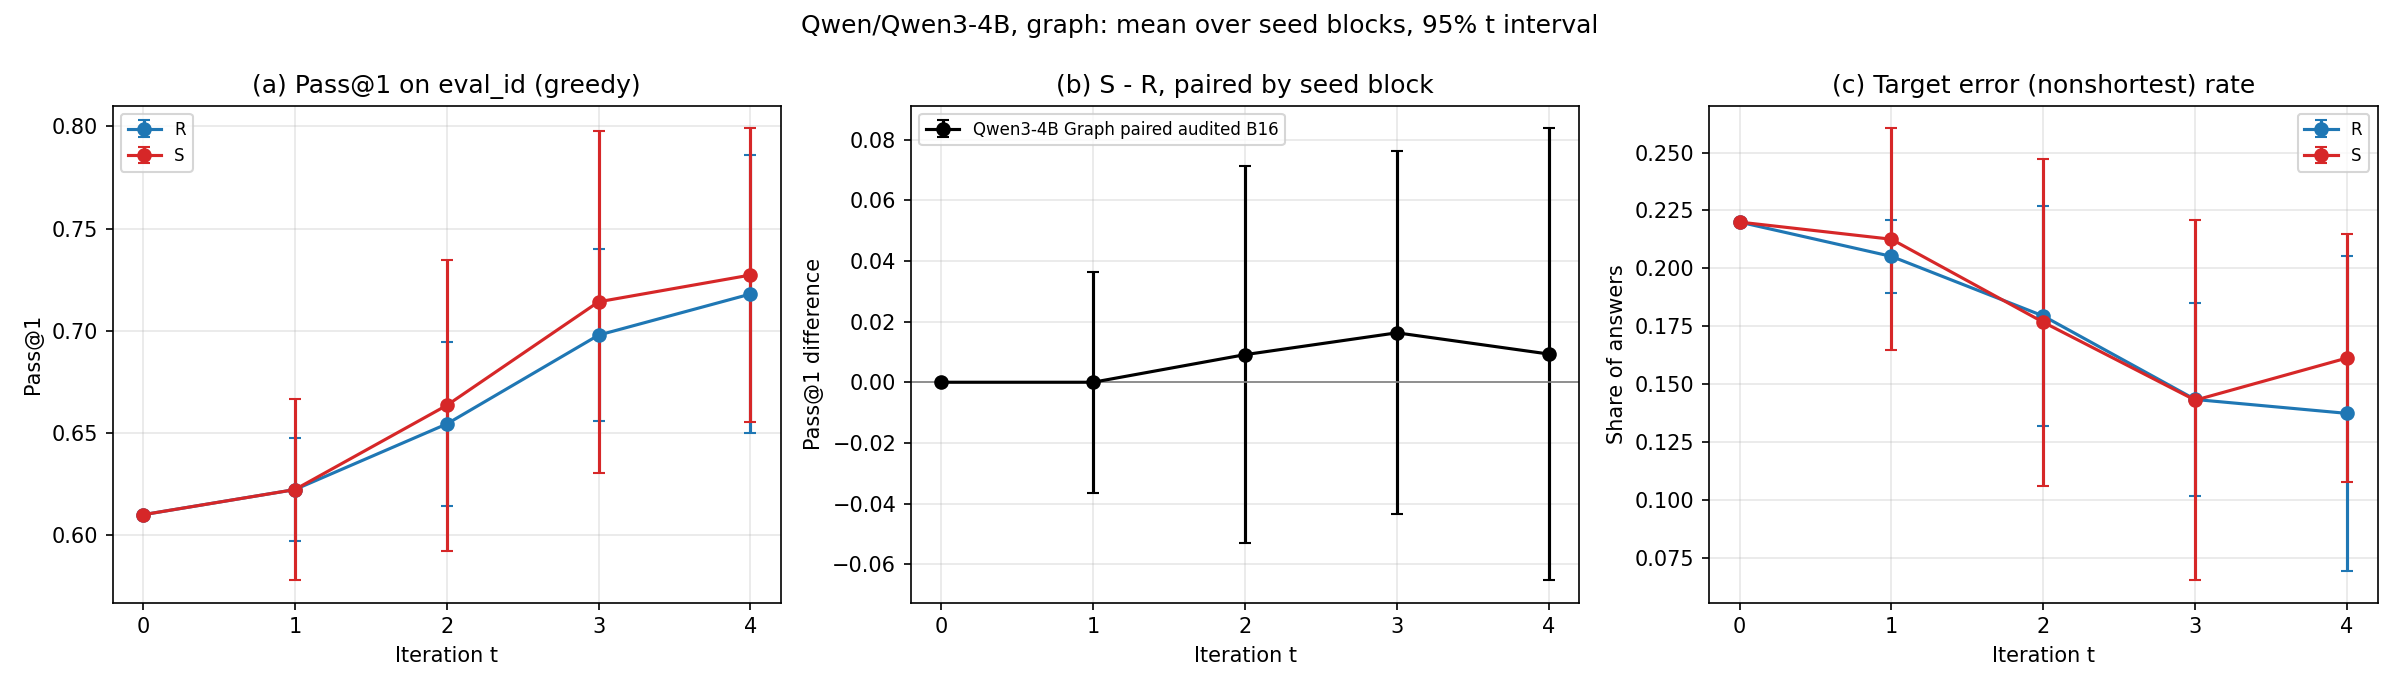
\includegraphics[width=0.90\linewidth]{figures/qwen4b_four_round_raw/audited_eval_id_pass1.png}
\par\smallskip
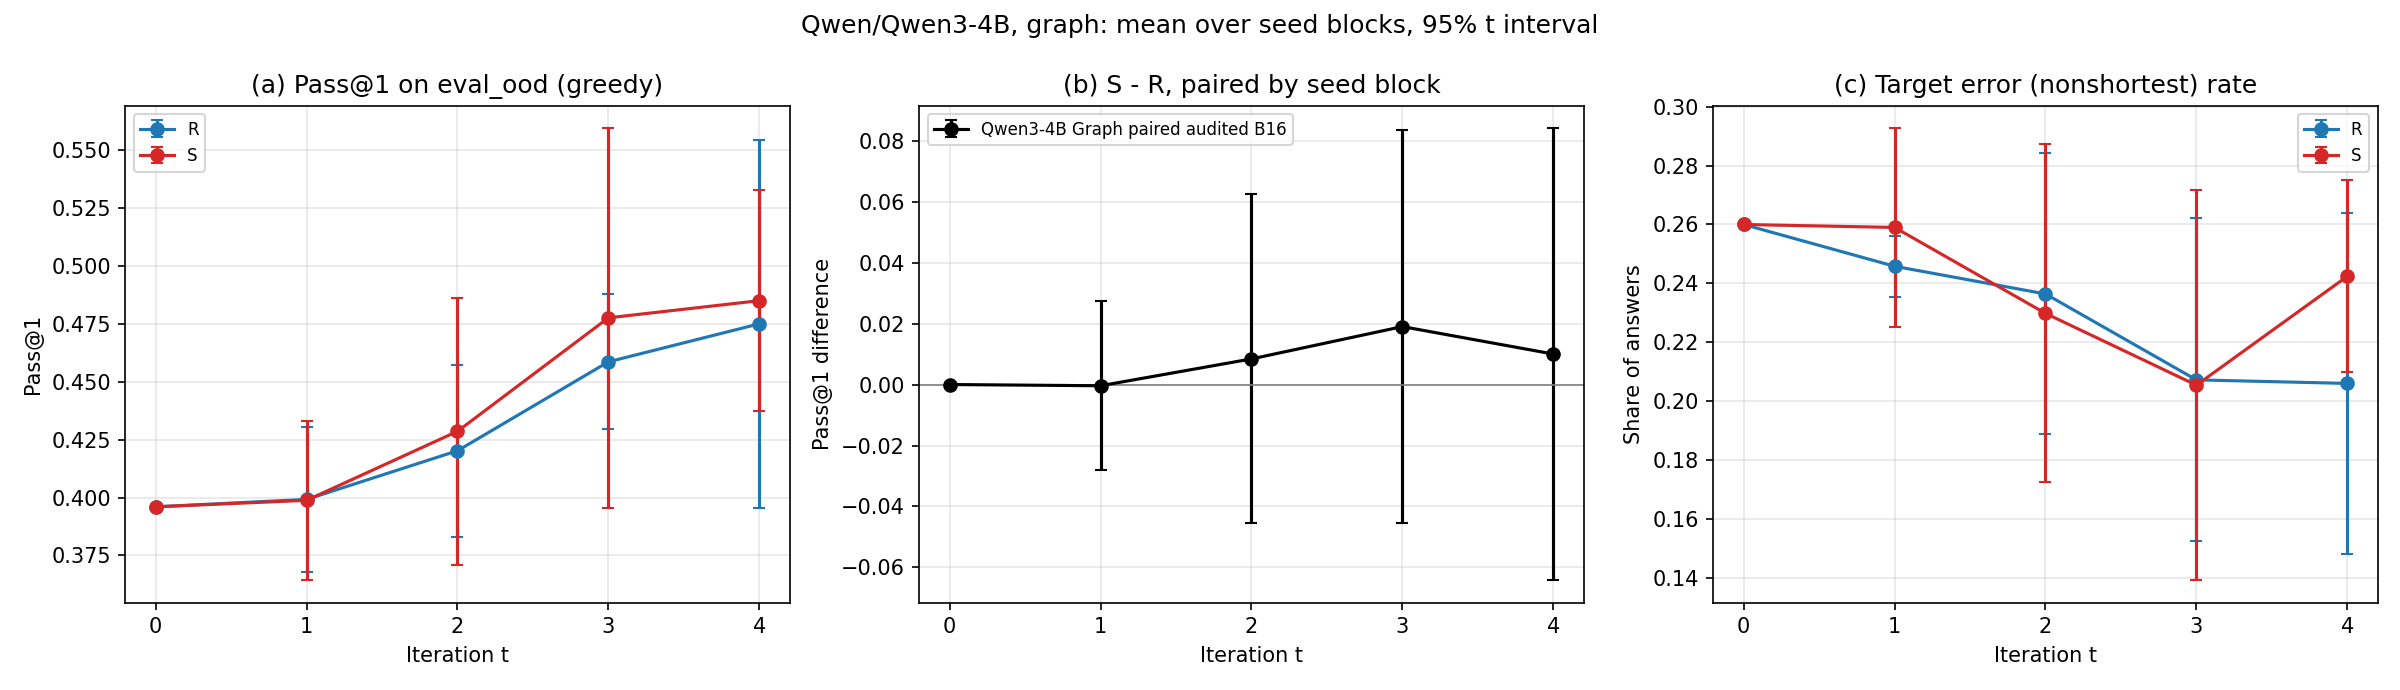
\includegraphics[width=0.90\linewidth]{figures/qwen4b_four_round_raw/audited_eval_ood_pass1.png}
\caption{Original adaptive-audit Qwen3-4B graph curves, ID (top)
and OOD (bottom), with 16 correctness queries per arm-round.
The panels show greedy Pass@1, paired $S-R$ accuracy, and
nonshortest-error incidence. Each audited arm spends 64 queries
over four rounds.}
\label{fig:qwen4b-raw-audited}
\end{figure}

Audited round-four $R/S$ accuracy is $0.7180/0.7273$ ID and
$0.4750/0.4850$ OOD, from audited-run bases $0.6100$ and $0.3960$.
The paired contrasts are $0.0093\pm0.0745$ and $0.0100\pm0.0741$.
They compare arms within the audited policy and
should not be interpreted as effects of auditing.

\begin{figure}[H]
\centering
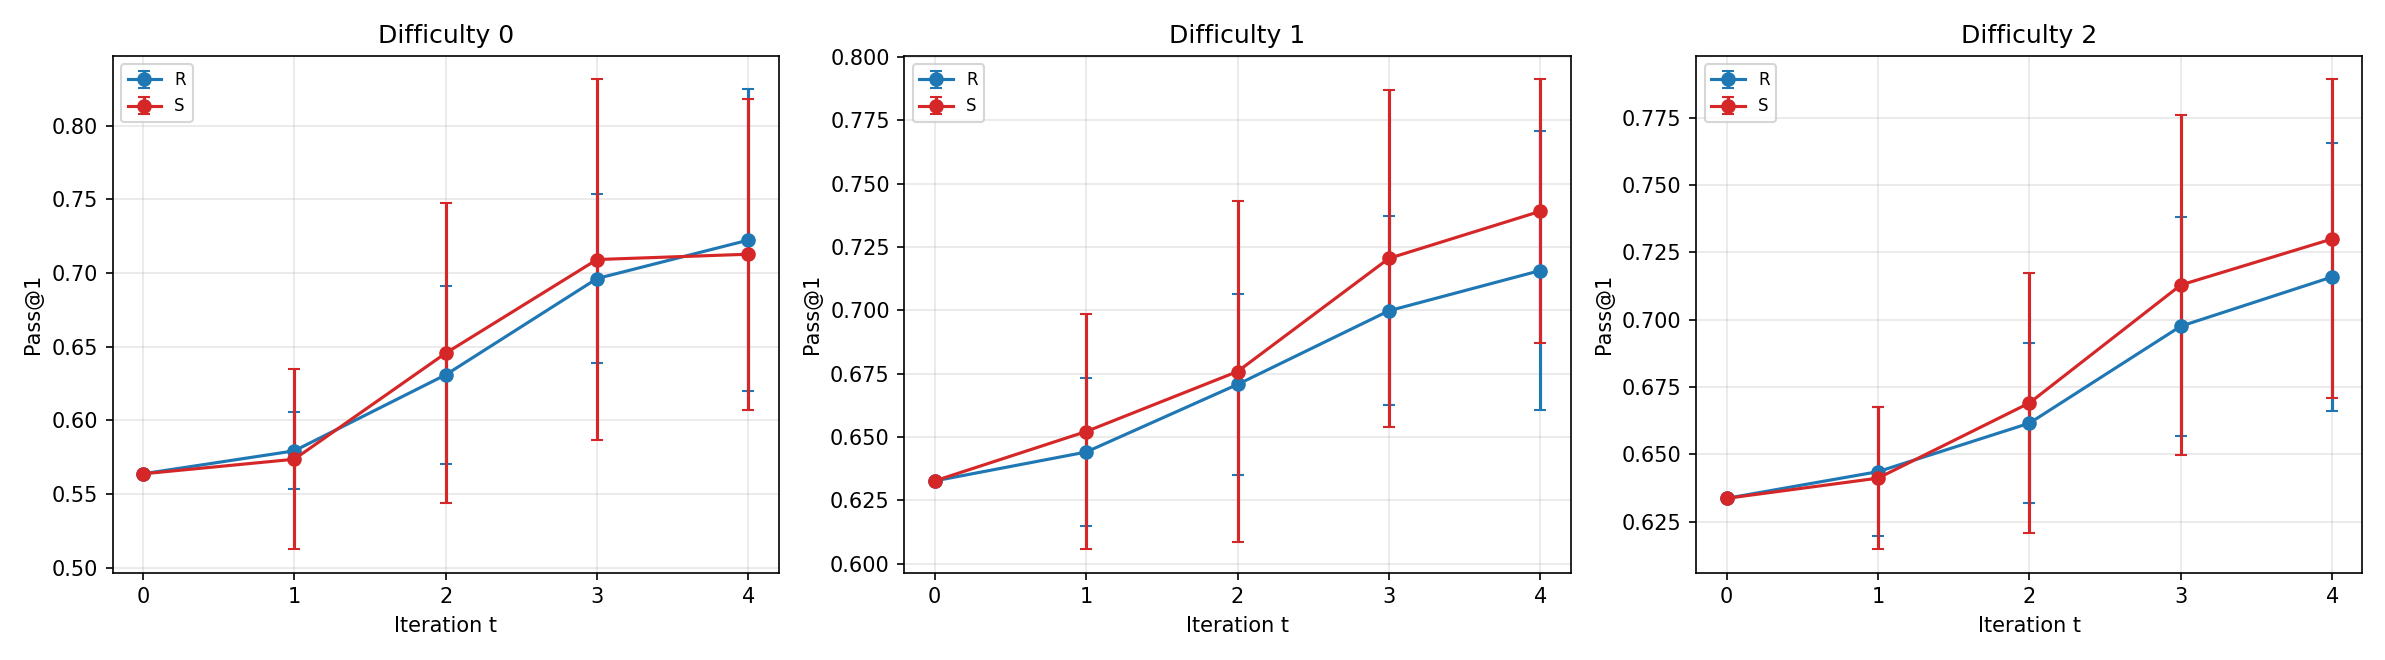
\includegraphics[width=0.90\linewidth]{figures/qwen4b_four_round_raw/audited_eval_id_by_difficulty.png}
\par\smallskip
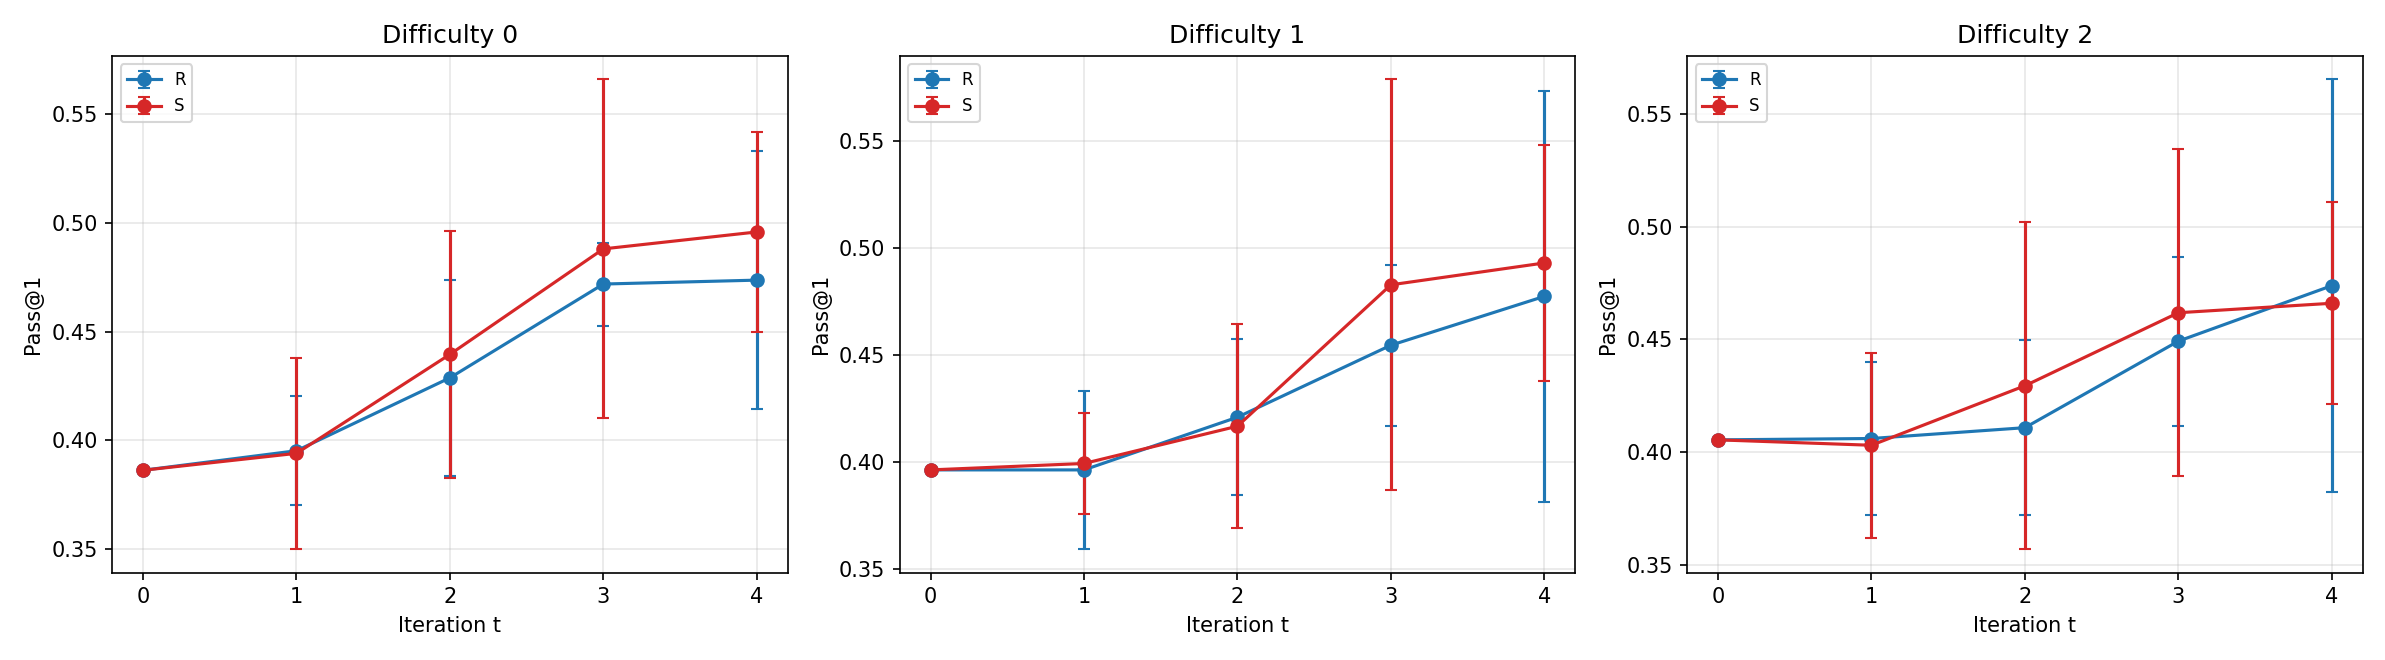
\includegraphics[width=0.90\linewidth]{figures/qwen4b_four_round_raw/audited_eval_ood_by_difficulty.png}
\caption{Original adaptive-audit Qwen3-4B graph accuracy by
generator stratum, ID (top) and OOD (bottom), for rounds 0--4.
Strata, fixed question sets, and interval conventions follow
Figure~\ref{fig:qwen4b-raw-unaudited-difficulty}.}
\label{fig:qwen4b-raw-audited-difficulty}
\end{figure}

The audited stratum curves use the same fixed questions and retain their
original panel-specific scales. They supplement the aggregate audited
results without establishing a stratum-specific audit benefit, which
would require a corresponding cross-policy comparison and treatment
of the multiple contrasts.

\begin{figure}[H]
\centering
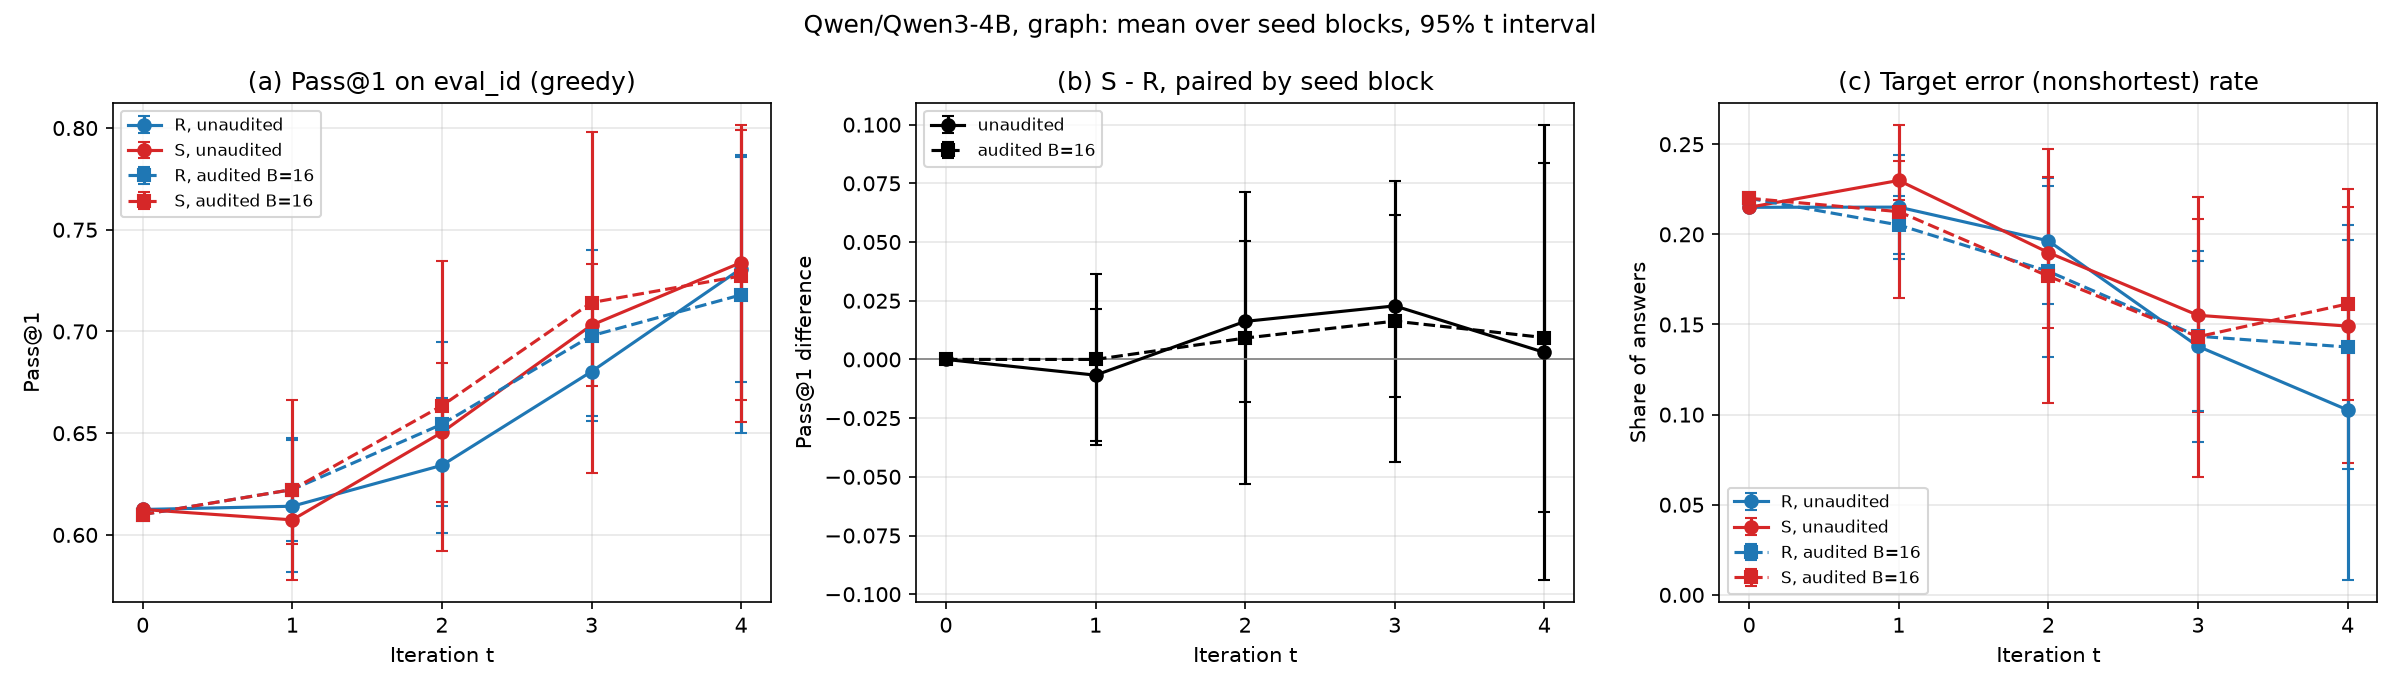
\includegraphics[width=0.90\linewidth]{figures/qwen4b_four_round_raw/comparison_eval_id_pass1.png}
\par\smallskip
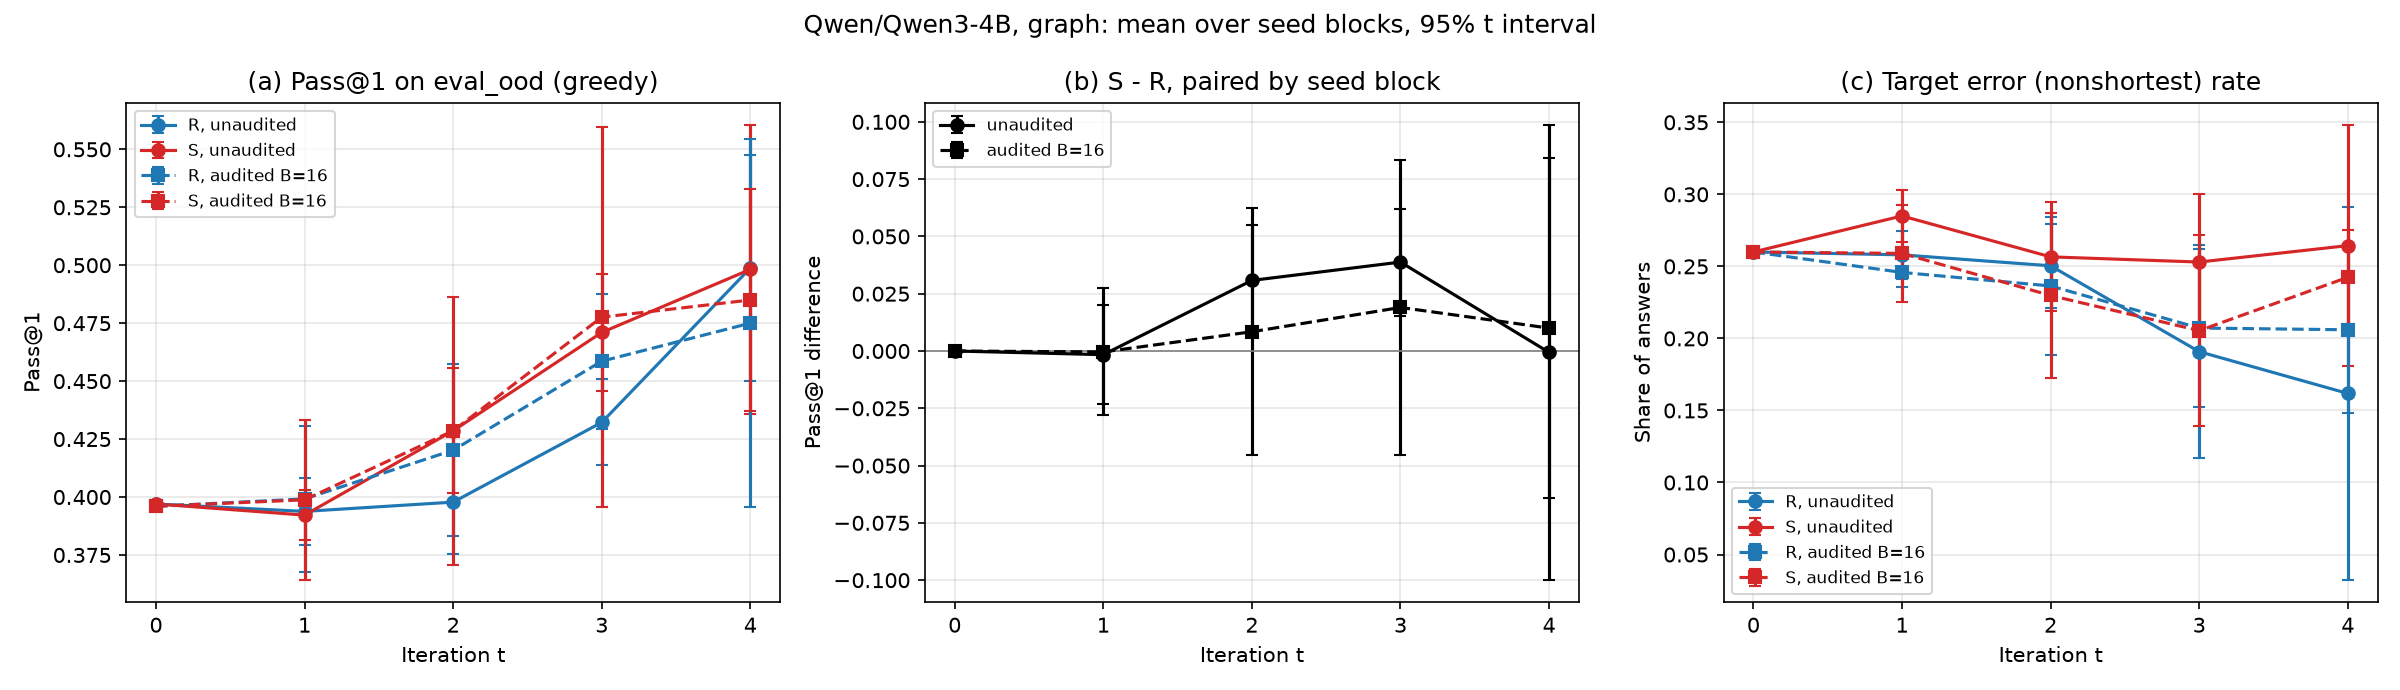
\includegraphics[width=0.90\linewidth]{figures/qwen4b_four_round_raw/comparison_eval_ood_pass1.png}
\caption{Joint Qwen3-4B graph trajectories, ID (top) and OOD
(bottom), generated with the original plotting method from the
same unaudited and audited checkpoints. The middle panels show
paired $S-R$ accuracy within each policy, not audited-minus-unaudited
effects.}
\label{fig:qwen4b-raw-comparison}
\end{figure}

Same-arm audit error changes are positive in mean
(Table~\ref{tab:audit-results}). Differences in optimizer effort
limit causal attribution: these results establish
neither an audit benefit nor a detrimental audit effect.

\begin{figure}[H]
\centering
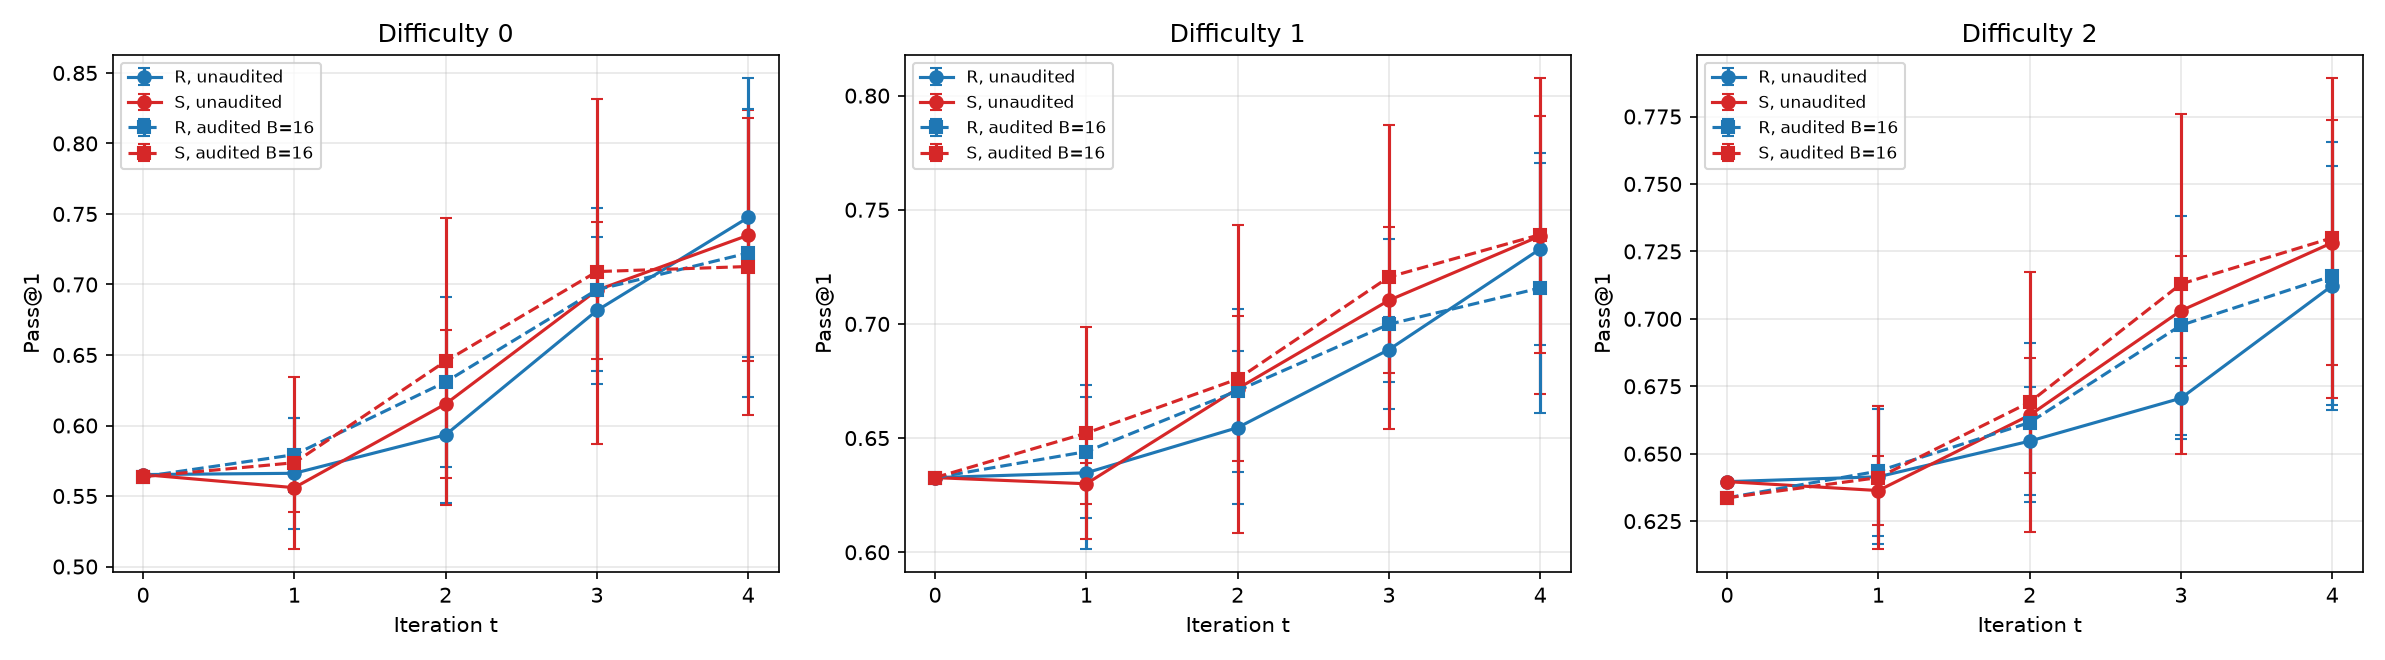
\includegraphics[width=0.90\linewidth]{figures/qwen4b_four_round_raw/comparison_eval_id_by_difficulty.png}
\par\smallskip
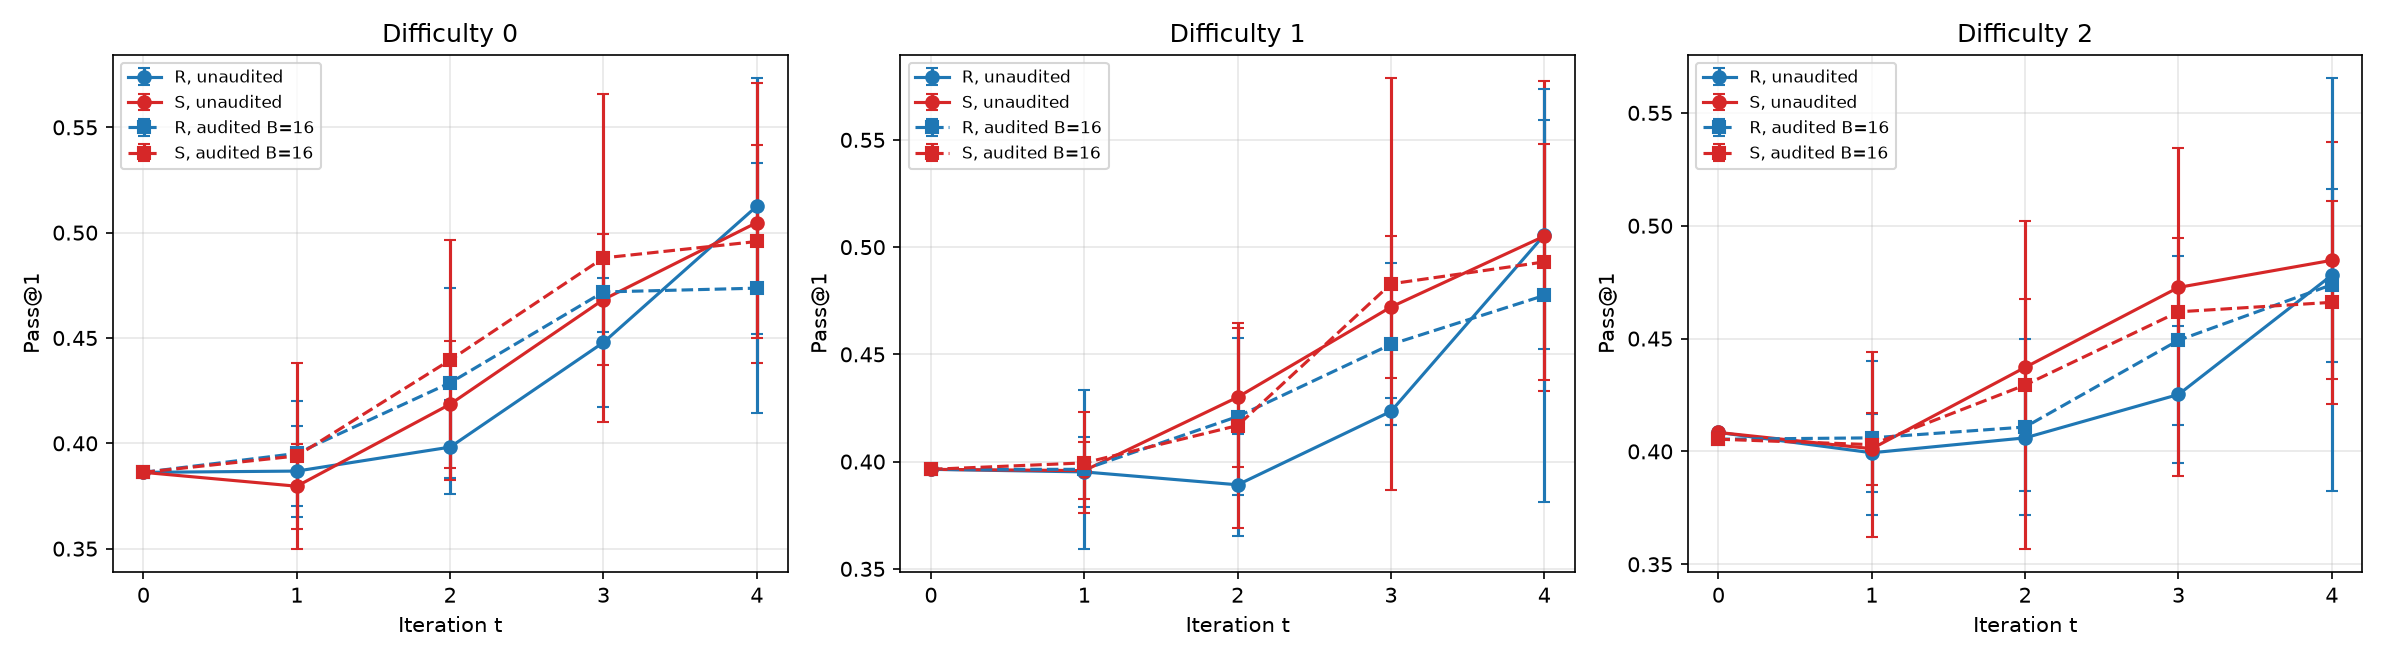
\includegraphics[width=0.90\linewidth]{figures/qwen4b_four_round_raw/comparison_eval_ood_by_difficulty.png}
\caption{Joint Qwen3-4B graph accuracy by generator stratum, ID
(top) and OOD (bottom), generated from the same checkpoint records
with the original plotting method. Both policies and arms use the
same question stratum at each checkpoint. Counts and interval
conventions follow Figure~\ref{fig:qwen4b-raw-unaudited-difficulty}.}
\label{fig:qwen4b-raw-comparison-difficulty}
\end{figure}

The two policies and arms share each question stratum. Panel-specific vertical scales are
unchanged, and the intervals are not adjusted across strata, rounds,
or policies. Consequently the joint breakdown remains descriptive,
consistent with the aggregate uncertainty rather than a separate
confirmatory analysis.
\endgroup
